\documentclass[conference]{IEEEtran}
\usepackage{fontspec}
\setmainfont{Times New Roman}
\setmonofont{Courier New}
\usepackage{graphicx}
\usepackage{booktabs}
\usepackage{amsmath}
\usepackage{amsfonts}
\usepackage{amssymb}
\usepackage{url}
\usepackage[hidelinks]{hyperref}
\usepackage{cite}
\usepackage{balance}
\setlength{\textfloatsep}{7pt plus 2pt minus 2pt}
\setlength{\floatsep}{7pt plus 2pt minus 2pt}
\setlength{\intextsep}{7pt plus 2pt minus 2pt}
\renewcommand{\IEEEbibitemsep}{0pt plus .5pt minus 1pt}

\begin{document}

\title{Ghép ảnh 2D từ video UAV có nhận thức rủi ro: Nghiên cứu thực nghiệm về chỉ báo, phân luồng và phục hồi}

\author{
\IEEEauthorblockN{Diệp Quang Sáng}
\IEEEauthorblockA{\small Trường Đại học FPT\\
TP.HCM, Việt Nam\\
diepqsang13@gmail.com}
\and
\IEEEauthorblockN{Nguyễn Đức Nam}
\IEEEauthorblockA{\small Trường Đại học FPT\\
TP.HCM, Việt Nam\\
namnguyen5406gl@gmail.com}
\and
\IEEEauthorblockN{Đào Đặng Nguyên Khôi}
\IEEEauthorblockA{\small Trường Đại học FPT\\
TP.HCM, Việt Nam\\
nguyenkhoidao2005@gmail.com}
\and
\IEEEauthorblockN{Trương Quang Đăng Khoa}
\IEEEauthorblockA{\small Trường Đại học FPT\\
TP.HCM, Việt Nam\\
Khoa2632006@gmail.com}
}

\maketitle

\begin{abstract}
Ghép ảnh 2D gia tăng từ video máy bay không người lái (UAV) dựa trên ước lượng homography tuần tự, vốn tích luỹ sai số trôi dạt khi các phép đăng ký cặp ảnh suy giảm trên địa hình nghèo đặc trưng hoặc lặp kết cấu. Bài báo trình bày một nghiên cứu thực nghiệm về các cơ chế nhận thức rủi ro trên 8 chuỗi bay UAV, phân tích 3.898 ảnh (3.890 cặp liên tiếp) trong đánh giá chuẩn bộ đối sánh và 3.899 ảnh (3.891 bước) trong đánh giá pipeline. Kết quả làm sáng tỏ ba câu hỏi nghiên cứu mà không đưa ra tuyên bố vượt trội tuyệt đối. Thứ nhất, phân tích mô tả cho thấy các chỉ báo đếm điểm có khả năng phân tách yếu đối với bất đồng cấp bước (tương quan Spearman vĩ mô $\rho = -0{,}091$ và $-0{,}127$; AUC vĩ mô $0{,}535$ và $0{,}557$), trong khi các thước đo hậu đăng ký---RMSE inlier ($\rho = 0{,}728$, AUC $0{,}882$), tỷ lệ pixel trắc quang lệch ngưỡng sau khi khử kỳ vọng ($\rho = 0{,}613$, AUC $0{,}834$) và độ tương quan chuẩn hoá ($\rho = -0{,}484$, AUC $0{,}762$)---tương quan chặt chẽ hơn với độ lệch tham chiếu. Thứ hai, bộ phân luồng hai tầng (SIFT leo thang sang SuperPoint-LightGlue) dưới kiểm định chéo LOSO với ngân sách huấn luyện $\le 25\%$ đạt sai số bước vĩ mô $2{,}940$\,px nhưng mất $813{,}70$\,s, so với $261{,}55$\,s khi chạy SuperPoint-LightGlue toàn bộ trên cấu hình phần cứng thử nghiệm. Thứ ba, dưới cùng ngưỡng kích hoạt, loại bỏ khung hình và neo lại keyframe chỉ giữ lại $43{,}42\%$ và $43{,}75\%$ số frame, trong khi tách mảnh giữ đủ toàn bộ frame nhưng làm vỡ hành trình thành $795$ mảnh độc lập. Kết quả chỉ rõ các đánh đổi thực tế giữa tỷ lệ lưu giữ, tính liên tục và thời gian thực thi.
\end{abstract}

\begin{IEEEkeywords}
Ghép ảnh video UAV, homography gia tăng, dự báo rủi ro, phân luồng thích ứng, lan truyền sai số, phân mảnh bản đồ, đánh giá chuẩn thực nghiệm.
\end{IEEEkeywords}

\section{Giới thiệu}
\label{sec:intro}

Tạo lập một bức ảnh ghép 2D không định toạ độ từ video độ cao thấp của máy bay không người lái (UAV) là giải pháp cung cấp thông tin không gian tức thời trong cứu hộ khẩn cấp, nông nghiệp và giám sát môi trường~\cite{hwang2026,li2023}. So với các quy trình tái dựng 3D đo ảnh (SfM) đòi hỏi tính toán đồ sộ, ghép ảnh gia tăng 2D liên kết tuần tự các phép biến đổi xạ ảnh phẳng (homography) giữa các khung hình video kế tiếp nhau~\cite{map2dfusion}.

Tuy nhiên, phương pháp ghép ảnh gia tăng tích luỹ sai số đăng ký theo thời gian. Trong một chuỗi gia tăng, toạ độ toàn cục của khung hình thứ $k$ được xác định thông qua phép nhân liên tiếp các ma trận homography bước:
\begin{equation}
H_{0 \leftarrow k} = H_{0 \leftarrow 1} H_{1 \leftarrow 2} \dots H_{k-1 \leftarrow k} = \prod_{j=1}^k H_{j-1 \leftarrow j}.
\label{eq:chain_accum_vi}
\end{equation}
Khi drone bay qua các khu vực nghèo kết cấu, thảm thực vật đồng nhất, hoặc góc bay gần như phẳng, quá trình đối sánh đặc trưng cặp ảnh có thể suy thoái. Nếu một ma trận homography $H_{k-1 \leftarrow k}$ thiếu chính xác được đưa vào chuỗi, các khung hình tiếp theo sẽ thừa hưởng sai số hình học đó, dẫn tới trôi dạt quỹ đạo tích luỹ và biến dạng trên canvas.

Để kiểm soát các rủi ro này, một hệ thống thực tế cần nhận thức rủi ro qua ba giai đoạn:
\begin{enumerate}
    \item \textbf{Dự báo / Phát hiện lỗi:} Xác định bước đăng ký cặp ảnh bị suy thoái trước khi biến đổi được tích lũy vào canvas toàn cục.
    \item \textbf{Phân luồng tài nguyên thích ứng:} Sử dụng bộ đối sánh cổ điển nhẹ theo mặc định và chỉ leo thang sang mô hình học sâu khi phát hiện rủi ro.
    \item \textbf{Phục hồi lỗi:} Kích hoạt chính sách can thiệp (bỏ khung hình, neo lại keyframe lịch sử, hoặc tách thành các mảnh bản đồ độc lập) khi phép ghép cặp thất bại.
\end{enumerate}

Các nghiên cứu tiền nhiệm đã đề xuất nhiều giải pháp cục bộ cho các thành phần này~\cite{hwang2026,li2023,kharismawati2025}, song mối quan hệ tương hỗ và các tương quan đánh đổi thực nghiệm giữa chúng cần được đánh giá một cách hệ thống. Nhiều hệ thống áp dụng tiêu chí chấp nhận dựa trên số lượng điểm khớp hoặc số lượng inlier của RANSAC~\cite{hwang2026}, với giả định rằng nhiều inlier đồng nghĩa với biến đổi phẳng tin cậy. Ngoài ra, các cơ chế phân luồng thường mặc định coi thuật toán cổ điển (như SIFT~\cite{lowe2004} hoặc ORB~\cite{rublee2011}) luôn nhanh hơn mô hình học sâu (như SuperPoint-LightGlue~\cite{detone2018,lindenberger2023} hoặc LoFTR~\cite{sun2021}), mà không xét tới sự hỗ trợ của phần cứng tăng tốc chuyên dụng.

Trong công trình này, chúng tôi tiến hành một nghiên cứu thực nghiệm về ghép ảnh UAV nhận thức rủi ro trên 8 chuỗi video từ bộ dữ liệu Map2DFusion~\cite{map2dfusion}. Chúng tôi tập trung giải quyết ba câu hỏi nghiên cứu:
\begin{itemize}
    \item \textbf{RQ1 (Dự báo lỗi):} Các chỉ báo cặp ảnh gọn nhẹ tương quan mô tả thế nào với bất đồng cấp bước trên các địa hình bay đa dạng, và các chỉ báo đếm điểm khác biệt thế nào so với các thước đo trắc quang và hình học hậu đăng ký?
    \item \textbf{RQ2 (Phân luồng thích ứng):} Bộ phân luồng hai tầng vận hành thế nào trên các chuỗi video mới dưới kiểm định chéo LOSO có ràng buộc ngân sách, và chi phí thời gian thực đo là bao nhiêu?
    \item \textbf{RQ3 (Phục hồi lỗi và phân mảnh):} Khi phát hiện rủi ro, các chính sách bỏ khung hình, neo lại keyframe và tách mảnh đánh đổi thế nào giữa tỷ lệ lưu giữ khung hình, tính liên tục của quỹ đạo và mức độ phân mảnh bản đồ?
\end{itemize}

Trên bộ dữ liệu này, các chỉ báo đếm điểm phân tách yếu hơn một số chỉ báo hậu đăng ký. Phân luồng đạt độ lệch bước trung bình vĩ mô thấp hơn SIFT trên tập bước có thể đánh giá của từng chính sách, nhưng chi phí tính toán cộng gộp bằng $3{,}11$ lần phương án chỉ dùng learned matcher. Split giữ đủ frame nhưng tạo 795 mảnh. Vì vậy, cần báo cáo đồng thời chất lượng, chi phí, tính khả dụng của phép đo và tính liên thông.

\section{Nghiên cứu liên quan}
\label{sec:related_work}

Ghép ảnh 2D gia tăng từ video máy bay không người lái (UAV) đòi hỏi giải quyết đồng thời bốn thách thức kỹ thuật: đăng ký chuỗi khung hình, giới hạn tài nguyên tính toán, phát hiện rủi ro lỗi đăng ký và kiểm soát lan truyền sai số. Phần này hệ thống hoá các công trình tiền nhiệm theo bốn hướng chính và xác lập phạm vi so sánh thực nghiệm của nghiên cứu.

\subsection{Ghép ảnh UAV gia tăng và SLAM đơn mục}
Các hệ thống ghép video UAV truyền thống và đương đại chủ yếu dựa trên luồng ước lượng xạ ảnh (homography) tuần tự. Hwang cùng cộng sự~\cite{hwang2026} phát triển hệ thống ghép ảnh trực giao 2D thời gian thực trên CPU, ước lượng ma trận homography gia tăng bằng các bộ trích xuất đặc trưng cổ điển (SIFT~\cite{lowe2004}, ORB~\cite{rublee2011}) kết hợp RANSAC~\cite{fischler1981}, sử dụng ngưỡng số lượng inlier cố định để kiểm duyệt biến đổi giữa các khung hình liên tiếp. Li cùng cộng sự~\cite{li2023} đề xuất khung ghép video gia tăng trong viễn thám UAV, ứng dụng tối ưu hoá sai số chiếu lại có trọng số, chọn khung hình chính (keyframe) theo tỷ lệ đè phủ quang học và cơ chế kết nối lại (rematch) với keyframe lịch sử nhằm giảm thiểu trôi dạt theo dõi. Chen cùng cộng sự~\cite{chen2022} xử lý biến dạng phối cảnh khi độ cao bay thay đổi thông qua quy hoạch động tìm đường nối tối ưu kết hợp phép biến đổi nửa xạ ảnh bảo toàn hình dạng. Nhằm khắc phục tính dễ tổn thương của chuỗi homography tuần tự, Bu cùng cộng sự~\cite{map2dfusion} giới thiệu Map2DFusion, kết hợp theo dõi trực tiếp mức pixel từ SLAM thị giác đơn mục với đồ thị keyframe và tối ưu hoá bundle adjustment cục bộ. Khác với các hệ thống SLAM thị giác toàn diện duy trì điểm bản đồ 3D và tối ưu hoá bundle adjustment, nghiên cứu của chúng tôi tập trung vào pipeline ghép ảnh 2D gia tăng bằng homography nhẹ vận hành dưới ràng buộc tài nguyên tuần tự mà không sử dụng tối ưu hoá đồ thị toàn cục.

\subsection{Đối sánh đặc trưng học sâu và ràng buộc tài nguyên}
Học sâu đã mang lại những bước tiến lớn trong đối sánh đặc trưng dưới sự thay đổi mạnh về điều kiện chiếu sáng và góc nhìn. DeTone cùng cộng sự~\cite{detone2018} giới thiệu SuperPoint, mạng tự giám sát để đồng thời phát hiện điểm đặc trưng và trích xuất vector mô tả. Lindenberger cùng cộng sự~\cite{lindenberger2023} phát triển LightGlue, mạng nơ-ron đồ thị tích hợp cơ chế loại bỏ điểm không khớp thích ứng và dừng sớm để tiết kiệm chi phí. Đối với hướng tiếp cận không dùng bộ dò điểm (detector-free), Sun cùng cộng sự~\cite{sun2021} xây dựng LoFTR dựa trên kiến trúc Transformer coarse-to-fine, trong khi Wang cùng cộng sự~\cite{wang2024} đề xuất Efficient LoFTR nhằm giảm độ phức tạp tính toán thông qua cơ chế chú ý tổng hợp (aggregated attention) với chọn lọc token thích ứng và tầng tương quan hai giai đoạn. Nhằm phục vụ các nền tảng biên, Potje cùng cộng sự~\cite{xfeat2024} thiết kế XFeat, kiến trúc đối sánh nhẹ tối ưu hoá riêng cho thiết bị bị giới hạn tài nguyên. Gần đây, Kim và Kim~\cite{kim2025} kết hợp trích xuất SIFT với bộ đối sánh LightGlue để xử lý các cặp ảnh UAV có góc xoay lớn.

Mặc dù các mô hình học sâu thể hiện năng lực đăng ký cặp ấn tượng, hành vi của chúng trong chuỗi video UAV liên tục bộc lộ những đánh đổi thực tế. Trong các chuỗi bay dài thiếu vắng bundle adjustment toàn cục, các biến đổi học sâu tuần tự vẫn có thể tích lũy sai số subpixel qua các bước bay danh định. Điều này đặt ra yêu cầu khảo sát các chiến lược kích hoạt có chọn lọc thay vì gọi mô hình sâu liên tục trên mọi bước.

\subsection{Dự báo lỗi đăng ký và ước lượng độ bất định}
Zaffar cùng cộng sự~\cite{zaffar2024} so sánh độ bất định dựa trên truy hồi, độ bất định aleatoric học từ dữ liệu và kiểm chứng hình học trong nhận diện địa điểm; đồng thời đề xuất một đường cơ sở sử dụng tư thế của ảnh tham chiếu. Mục tiêu của họ là độ tin cậy của kết quả truy hồi ảnh, không phải drift tích lũy của mosaic UAV; vì vậy cần đánh giá chỉ báo bằng một thước đo thay thế lỗi đăng ký được định nghĩa rõ. Barath cùng cộng sự~\cite{barath2023} cung cấp homography tham chiếu để đánh giá bộ ước lượng bền vững và phương pháp lọc tương ứng điểm. Ivashechkin cùng cộng sự~\cite{ivashechkin2021} giới thiệu VSAC, sử dụng khái niệm inlier độc lập và kiểm tra giả thuyết tuần tự thích ứng để cải thiện ước lượng bền vững. Các công trình này phân biệt đánh giá độ tin cậy và ước lượng bền vững với bài toán quản lý một phép biến đổi đã được chấp nhận trong chuỗi dài.

Đầu ra nội tại của bộ ước lượng là tín hiệu hữu ích khi chấp nhận phép đăng ký~\cite{hwang2026,li2023}, nhưng phần dư nhỏ trên tập correspondence được chọn không tự chứng minh tính nhất quán toàn cục. Nghiên cứu này khảo sát liệu tính nhất quán diện mạo hậu đăng ký và chỉ báo hình học có bổ sung bằng chứng mô tả ngoài số điểm hay không; không giả định nhất quán trắc quang chứng minh hình học đúng.

\subsection{Lan truyền sai số chuỗi và chính sách phục hồi}
Khi xảy ra suy giảm chất lượng đăng ký, hệ thống ghép ảnh gia tăng cần một chính sách phục hồi để xử lý bước lỗi. Giải pháp đơn giản nhất là loại bỏ khung hình (frame dropping) kém tin cậy~\cite{hwang2026}. Tuy nhiên, việc loại bỏ khung hình làm nới rộng khoảng cách thời gian giữa khung hình mới và điểm neo hiện thời của bản đồ, làm tăng độ lệch phối cảnh và có thể dẫn đến các bước loại bỏ tiếp theo. Li cùng cộng sự~\cite{li2023} giải quyết vấn đề này bằng cách tìm kiếm các keyframe trong quá khứ để đối sánh lại, dù khả năng kết nối lại phụ thuộc vào độ đè phủ không gian và giới hạn cửa sổ tìm kiếm. Kharismawati và Kazic~\cite{kharismawati2025} phát triển pipeline DroneZaic cho video UAV nông nghiệp, sử dụng phân cụm chuyển động để chia chuyến bay thành các mảnh độc lập (submosaics).

Chiến lược tách mảnh bảo toàn toàn bộ số lượng khung hình gốc bằng cách mở điểm neo tham chiếu mới khi gặp đứt gãy đăng ký, song bản chất là đánh đổi tính liên tục của bề mặt bản đồ đơn nhất lấy độ bao phủ cục bộ. Ngược lại, chiến lược loại bỏ khung hình duy trì tính liền mạch của chuỗi sống sót nhưng có nguy cơ loại bỏ phần lớn hành trình bay khi tình trạng suy giảm kéo dài. Trong nghiên cứu này, chúng tôi so sánh các chính sách phục hồi trên dưới các tiêu chí kích hoạt rủi ro thống nhất.


\section{Mô hình cơ sở và phương pháp luận}
\label{sec:methodology}

\subsection{Pipeline homography gia tăng cơ sở}
\label{subsec:baseline_model}

Quy trình ghép ảnh 2D cơ sở sử dụng mô hình xạ ảnh phẳng~\cite{map2dfusion,hwang2026}. Ký hiệu $I_k$ là khung hình thứ $k$. Với mỗi cặp khung hình liên tiếp $(I_{k-1}, I_k)$, các điểm đặc trưng và vector mô tả được trích xuất và đối sánh. Với tập tương ứng $(p_{k-1}^j, p_k^j)$, ma trận homography $H_{k-1 \leftarrow k} \in \mathbb{R}^{3 \times 3}$ được ước lượng bằng RANSAC~\cite{fischler1981} với ngưỡng sai số chiếu lại $3{,}0$\,px:
\begin{equation}
p_{k-1}^j \approx \pi(H_{k-1 \leftarrow k} \tilde{p}_k^j),
\label{eq:homography_proj_vi}
\end{equation}
trong đó $\tilde{p} = [u, v, 1]^T$ biểu diễn toạ độ thuần nhất và $\pi([x, y, z]^T) = [x/z, y/z]^T$ biểu diễn phép chiếu thuần nhất.

Phép chuyển về độ phân giải gốc dùng $D=\operatorname{diag}(W/w,H/h,1)$, trong đó $(w,h)$ và $(W,H)$ là kích thước ảnh xử lý và ảnh gốc: $H_{\mathrm{orig}}=D H D^{-1}$. Các kiểm tra chấp nhận số học và hình học trong benchmark không chứng minh phép đăng ký đúng trên toàn cảnh.

Toạ độ canvas toàn cục được tạo thành bằng cách tích luỹ các biến đổi hợp lệ qua Eq.~\eqref{eq:chain_accum_vi}. Một phép tịnh tiến affine $T$ dịch chuyển gốc toạ độ $H_{0 \leftarrow k}$ về miền không âm trên canvas. Vùng ảnh đè phủ được hoà trộn bằng phương pháp lấy trung bình 50/50 trên canvas.

\begin{figure*}[t]
\centering
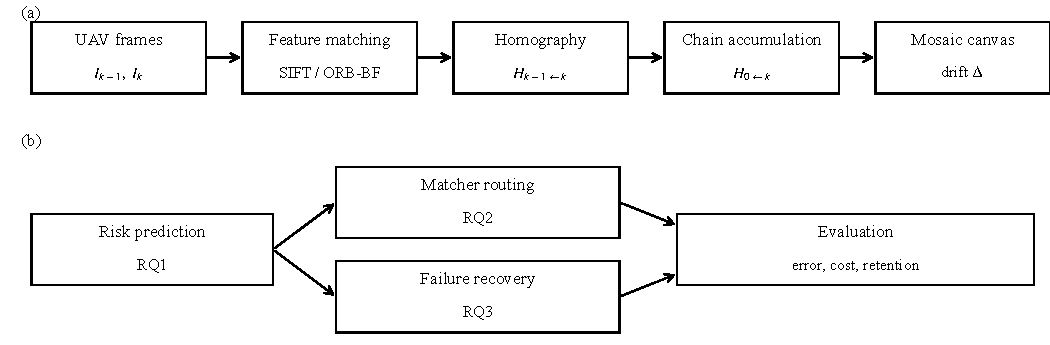
\includegraphics[width=0.96\textwidth]{figures/baseline.pdf}
\caption{Kiến trúc hệ thống thực nghiệm. Khung (a) minh hoạ pipeline ghép ảnh 2D tuần tự cơ sở không có can thiệp nhận thức rủi ro, nơi sai số đăng ký tích luỹ không kiểm soát vào canvas toàn cục. Khung (b) minh hoạ các can thiệp mô-đun được đánh giá: phát hiện rủi ro cấp bước (RQ1), phân luồng thích ứng hai tầng dưới kiểm định chéo LOSO (RQ2), và các chính sách phục hồi hạ nguồn (RQ3: none, drop, anchor, split) dưới cùng một ngưỡng kích hoạt thống nhất.}
\label{fig:baseline_arch}
\end{figure*}

\subsection{Quan sát thực nghiệm cơ sở gốc và pilot học sâu}
\label{subsec:native_baseline}

Để xác lập mốc so sánh thực nghiệm, chúng tôi xem xét kết quả thực thi cơ sở trên chuỗi \texttt{village} gồm 406 khung hình ở độ phân giải gốc $1920 \times 1080$. Bảng~\ref{tab:native_pilot} tổng hợp kết quả giữa SIFT-BF, ORB-BF và các thử nghiệm pilot học sâu SIFT-LightGlue, SuperPoint-LightGlue.

\begin{table*}[t]
\centering
\caption{So sánh Baseline và Deep Pilot trên chuỗi \texttt{village} (406 khung hình, độ phân giải gốc)}
\label{tab:native_pilot}
\footnotesize
\begin{tabular}{lcccc}
\toprule
Cấu hình & Số frame ghép & Tổng thời gian (s) & Phạm vi đồng hồ & Độ phủ canvas \\
\midrule
SIFT-BF (B) & 406 / 406 & 858{,}88 & Toàn bộ pipeline & -- \\
ORB-BF (B) & 406 / 406 & 231{,}72 & Toàn bộ pipeline & -- \\
SIFT-LG (P) & 406 / 406 & 1292{,}46 & Tổng chuỗi & 82{,}45\% \\
SP-LG (P) & 406 / 406 & 512{,}40 & Tổng chuỗi & 75{,}15\% \\
\bottomrule
\end{tabular}
\end{table*}

\begin{figure*}[t]
\centering
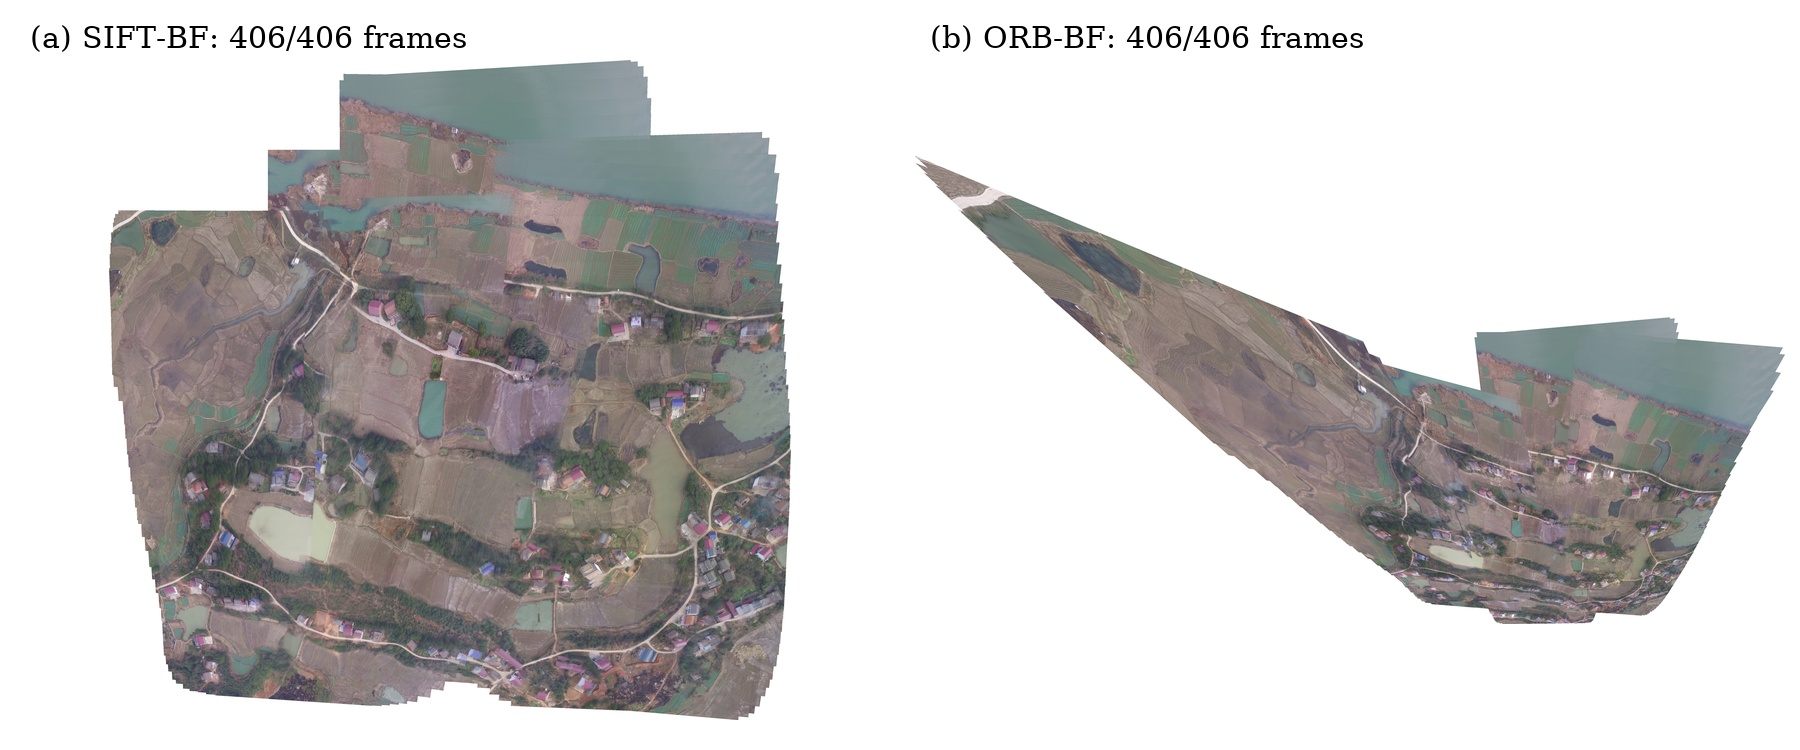
\includegraphics[width=0.88\textwidth]{figures/baseline_mosaics.jpg}
\caption{So sánh định tính các baseline ghép ảnh cổ điển trên chuỗi bay \texttt{village} (406 khung hình). Khung (a) là kết quả của SIFT-BF ($406/406$ khung hình, thời gian $858{,}88$\,s), xuất hiện các vết nối quang học và méo nhẹ cục bộ. Khung (b) là kết quả của ORB-BF ($406/406$ khung hình, thời gian $231{,}72$\,s), bị biến dạng kéo dài và méo phi tuyến tại các khúc cua của drone. Cả hai đều ghép đủ $100\%$ khung hình, chứng minh rằng tỷ lệ giữ frame chưa phản ánh đầy đủ độ chính xác hình học.}
\label{fig:baseline_mosaics}
\end{figure*}

Cả hai baseline cổ điển đặt đủ $406/406$ frame nhưng canvas đã lưu có hình dạng khác nhau và đường nối nhìn thấy được (Hình~\ref{fig:baseline_mosaics}); retention không chứng minh độ chính xác hình học. Pilot learned báo độ phủ canvas $82{,}45\%$ (SIFT-LG) và $75{,}15\%$ (SP-LG). Đồng hồ tổng chuỗi không chỉ đo matching và không gồm pilot cặp ảnh riêng. Các bản ghi ảnh gốc khác nhau về thực thi và phạm vi đo nên không phải phép so sánh tăng tốc có kiểm soát với benchmark 640\,px.

\subsection{Các chỉ báo rủi ro cấp cặp ảnh (RQ1)}
\label{subsec:indicators}

Để phát hiện suy thoái đăng ký ở cấp bước, chúng tôi đánh giá 8 chỉ báo:
\begin{enumerate}
    \item \textbf{Chỉ báo đếm điểm:} Số lượng match thô ($N_m$), số lượng inlier RANSAC ($N_{in}$), và tỷ lệ inlier $R_{in} = N_{in} / \max(N_m, 1)$.
    \item \textbf{Phân bố hình học:} Tỷ lệ diện tích bao lồi inlier ($\mathcal{A}_{hull} / (w \cdot h)$) và tỷ lệ đè phủ diện tích bao của hai khung hình ($\mathcal{O}_{area} / (w \cdot h)$).
    \item \textbf{Nhất quán hậu đăng ký:} Sai số chiếu lại RMSE inlier theo công thức:
    \begin{equation}
    \text{RMSE} = \sqrt{\frac{1}{N_{in}} \sum_{j=1}^{N_{in}} \| p_{k-1}^j - \pi(H_{k-1 \leftarrow k} \tilde{p}_k^j) \|_2^2},
    \label{eq:rmse_inlier_vi}
    \end{equation}
    và các thước đo trắc quang trên miền đè phủ sau khi biến đổi ngược $I_{k-1}$ sang toạ độ $I_k$ qua $H^{-1}$. Trên mặt nạ đè phủ $M$, cường độ xám $x$ (ảnh biến đổi) và $y$ (ảnh đích) được trừ kỳ vọng trung bình ($x_p' = x_p - \bar{x}$, $y_p' = y_p - \bar{y}$). Độ tương quan chuẩn hoá (photo NCC) và tỷ lệ pixel trắc quang lệch ngưỡng (photo bad fraction, chênh lệch tuyệt đối vượt 25 mức) được tính theo:
    \begin{align}
    \text{NCC}(x, y) &= \frac{\sum_{p \in M} x_p' y_p'}{\sqrt{\sum_{p \in M} (x_p')^2 \sum_{p \in M} (y_p')^2} + 10^{-9}}, \label{eq:ncc_vi} \\
    \text{Frac}_{bad} &= \frac{1}{|M|} \sum_{p \in M} \mathbb{I}(|x_p' - y_p'| > 25). \label{eq:photo_bad_vi}
    \end{align}
    Nếu miền đè phủ rỗng ($|M| = 0$), giá trị mặc định là $\text{NCC} = 0{,}0$ và $\text{Frac}_{bad} = 1{,}0$.
\end{enumerate}

\subsection{Phân luồng thích ứng dưới kiểm định chéo LOSO (RQ2)}
\label{subsec:routing_method}

Chính sách phân luồng hai tầng gồm:
\begin{itemize}
    \item \textbf{Tầng 1 (Mặc định):} SIFT-BF trên ảnh cạnh dài 640\,px.
    \item \textbf{Tầng 2 (Leo thang):} SuperPoint-LightGlue học sâu~\cite{detone2018,lindenberger2023}.
\end{itemize}
Đối chứng learned-only dùng Tầng 2 ở mọi bước. Routed-FR giữ nguyên quyết định leo thang nhưng chạy learned matcher trên ảnh gốc ở các bước leo thang thay cho phiên bản 640\,px.

Một bước kích hoạt leo thang lên Tầng 2 nếu thoả mãn bất kỳ điều kiện rủi ro nào:
\begin{equation}
\begin{aligned}
\text{Trigger}(k)={}&(\text{status}\neq\text{success})\\
 &\lor(\text{NCC}<\tau_{\mathrm{ncc}})\lor(R_{in}<0{,}30).
\end{aligned}
\label{eq:risk_trigger_vi}
\end{equation}

Dưới kiểm định chéo LOSO trên 8 chuỗi, chuỗi $s$ được giữ lại làm tập kiểm thử. Ngưỡng $\tau_{\mathrm{ncc}}$ được chọn từ tập lưới $\{0{,}90; 0{,}92; 0{,}93; 0{,}94; 0{,}95; 0{,}96; 0{,}97; 0{,}98; 0{,}99\}$ trên 7 chuỗi huấn luyện dưới ràng buộc:
\begin{equation}
\tau_{\mathrm{ncc}}^* = \max \left\{ \tau \;\middle|\; \text{Escalation}(s_{train}) \le 25\%, \; \forall s_{train} \right\}.
\label{eq:loso_budget_vi}
\end{equation}
Nếu tập ngưỡng khả thi rỗng, fold được ghi là \texttt{infeasible}; đánh giá chẩn đoán dùng ngưỡng dự phòng cấu hình $\tau_{\mathrm{ncc}}=0{,}95$ mà không tuyên bố tuân thủ ngân sách. Cả 8 fold được báo cáo đều có ngưỡng khả thi trên tập huấn luyện và áp dụng nguyên ngưỡng đó lên chuỗi kiểm thử. NCC hoặc tỷ lệ inlier bị thiếu cũng kích hoạt leo thang.

\subsection{Các chính sách phục hồi lỗi hạ nguồn (RQ3)}
\label{subsec:recovery_method}

Khi một bước được gắn cờ rủi ro theo Eq.~\eqref{eq:risk_trigger_vi}, pipeline kích hoạt chính sách phục hồi. Chúng tôi khảo sát bốn chính sách trên matcher cố định:
\begin{enumerate}
    \item \textbf{None (Chấp nhận):} Tiếp tục xâu chuỗi biến đổi nếu phép đối sánh thành công, bỏ qua cờ rủi ro.
    \item \textbf{Drop (Bỏ qua):} Bỏ frame $I_k$ và thử đăng ký frame tiếp theo về frame được đặt gần nhất; sau các lần bỏ trước đó, mốc này không nhất thiết là $I_{k-1}$.
    \item \textbf{Anchor (Neo lại):} Thử ba frame đã đặt gần nhất, loại trừ frame được đặt cuối cùng. Chỉ số các frame này không nhất thiết liên tiếp.
    \item \textbf{Split (Tách mảnh):} Mở chuỗi biến đổi mới với frame $I_k$ làm gốc. Run F ghi vị trí đặt và ma trận biến đổi, không dựng canvas cho từng chính sách phục hồi.
\end{enumerate}
RQ3 được đánh giá trên matcher cố định (SIFT-BF cho 7 cảnh, EfficientLoFTR cho grass), không phải là pipeline tích hợp nối tiếp trực tiếp từ kết quả phân luồng RQ2.

\section{Đối sánh tham chiếu và giao thức thực nghiệm}
\label{sec:protocol}

\subsection{Tập dữ liệu và kiểm kê số liệu đầu vào}
\label{subsec:datasets}

Thực nghiệm sử dụng bộ dữ liệu Map2DFusion~\cite{map2dfusion} gồm 8 chuỗi video: \texttt{monticules}, \texttt{npu}, \texttt{saplings}, \texttt{centralPark}, \texttt{factory}, \texttt{grass}, \texttt{huangqi} và \texttt{village}. Dữ liệu quỹ đạo và thông số mặt phẳng bay có trong gói dữ liệu nhưng có chủ đích không sử dụng trong nghiên cứu này để tập trung đo lường tính tự nhất quán từ hình ảnh.

\begin{table}[h]
\centering
\caption{Kiểm kê tập dữ liệu và thông số các chuỗi thực nghiệm}
\label{tab:sequences}
\footnotesize
\begin{tabular}{lrrrr}
\toprule
Sequence & M frames & F frames & Common & Invalid \\
\midrule
monticules & 395 & 395 & 11 & 0 \\
npu & 337 & 337 & 16 & 0 \\
saplings & 482 & 482 & 12 & 0 \\
centralPark & 835 & 836 & 35 & 1 \\
factory & 402 & 402 & 7 & 4 \\
grass & 648 & 648 & 6 & 84 \\
huangqi & 393 & 393 & 27 & 0 \\
village & 406 & 406 & 24 & 0 \\
\bottomrule
\end{tabular}

\end{table}

Ảnh có cạnh dài tối đa 640\,px, kích thước chia hết cho 32 (ví dụ $1920\times1080$ thành $640\times352$). M ghi ngân sách 2.000 keypoint cho bộ trích xuất thưa, ngưỡng ratio BF 0,75, ngưỡng RANSAC 3\,px và ngưỡng confidence EfficientLoFTR 0,2.

Bảng~\ref{tab:sequences} kiểm kê chi tiết số lượng khung hình:
\begin{itemize}
    \item Benchmark M gồm \textbf{3.898 ảnh} và \textbf{3.890 cặp liên tiếp}.
    \item Pipeline F gồm \textbf{3.899 ảnh} và \textbf{3.891 bước}.
\end{itemize}
Sự chênh lệch một ảnh xuất phát từ việc pipeline F giữ lại file trùng lặp trong \texttt{centralPark}: \nolinkurl{1454510665.360000 (1).jpg}, có mã băm SHA-256 trùng với file gốc. M đã loại bỏ file này, còn F xử lý nó. Toàn bộ 3.898 ảnh còn lại đều khớp mã băm trên cả hai run.

\subsection{Đối sánh tham chiếu và cổng kiểm duyệt}
\label{subsec:ref_gating}

Khi không sử dụng toạ độ thực địa bên ngoài, chúng tôi sử dụng bộ đối sánh tham chiếu: SIFT ở độ phân giải gốc (4.000 điểm đặc trưng, ratio test 0,75, RANSAC 3,0\,px).

Để kiểm soát chất lượng tham chiếu, chúng tôi áp dụng \textbf{Cổng kiểm duyệt tham chiếu}: homography $H_{ref}$ chỉ được chấp nhận nếu đạt $\ge 100$ inlier. Nếu dưới 100 inlier, bước đó bị đánh dấu \texttt{invalid} ($89$ bước trong F, trong đó có 84 bước ở \texttt{grass}). Sai số bước chỉ tính trên các bước tham chiếu hợp lệ.

\section{Công thức toán học của các thước đo}
\label{sec:metrics}

\subsection{Bất đồng đăng ký cấp bước}
\label{subsec:metric_step_error}

Ký hiệu $H_{est}$ là homography ước lượng đưa về độ phân giải gốc và $H_{ref}$ là homography tham chiếu hợp lệ. Độ phân kỳ hình học được đo trên 5 điểm mốc pixel $\mathcal{S} = \{ (0, 0), (W, 0), (W, H), (0, H), (W/2, H/2) \}$ gồm 4 góc và tâm ảnh:
\begin{equation}
E_{step}(H_{est}, H_{ref}) = \frac{1}{5} \sum_{p \in \mathcal{S}} \| \pi(H_{est} \tilde{p}) - \pi(H_{ref} \tilde{p}) \|_2.
\label{eq:step_error_vi}
\end{equation}
Một bước bị coi là bất đồng nếu $E_{step} > 2{,}0$\,px. Trên 3.794 bước đánh giá hợp lệ, có 1.075 bước ($28{,}33\%$) vượt ngưỡng này đối với SIFT cổ điển.
RQ1 tính tương quan Spearman và ROC-AUC theo từng chuỗi rồi lấy trung bình vĩ mô. Chiều điểm rủi ro được xác định trước theo ý nghĩa chỉ báo (RMSE/photo bad fraction lớn hơn; số điểm/tỷ lệ/NCC nhỏ hơn), không đảo AUC hậu nghiệm để vượt 0,5. AUC không xác định trên chuỗi chỉ có một lớp.

\subsection{Độ trôi ATE chuỗi vs trực tiếp trên khung hình chung}
\label{subsec:metric_ate}

Để đánh giá độ trôi tích luỹ, chúng tôi áp dụng phương pháp \textbf{Đo tự nhất quán Chain-vs-Direct}. Với khung hình $k$, homography chuỗi $H_{0 \leftarrow k}^{chain}$ được so sánh với homography đăng ký trực tiếp $H_{0 \leftarrow k}^{direct}$ về frame 0 bằng SIFT ảnh gốc.

\textbf{Tập khung hình chung hợp lệ} $\mathcal{C}$ là tập hợp các khung hình thoả mãn:
\begin{enumerate}
    \item Đăng ký trực tiếp $H_{0 \leftarrow k}^{direct}$ đạt $\ge 100$ inlier.
    \item Cả 7 bộ đối sánh đều giữ chuỗi không gãy tới frame $k$.
\end{enumerate}
Tập chung loại frame 0 và được xác định riêng cho từng chuỗi; tổng cộng có 138 frame hợp lệ. Đặt $e_k=E_{step}(H_{0\leftarrow k}^{chain},H_{0\leftarrow k}^{direct})$. Common ATE trong artifact là căn trung bình bình phương theo miền pixel:
\begin{equation}
\text{ATE}_{common}=\sqrt{|\mathcal{C}|^{-1}\sum_{k\in\mathcal{C}}e_k^2}.
\label{eq:common_ate_vi}
\end{equation}
Đây là độ bất đồng phép biến đổi ảnh, không phải sai số quỹ đạo ground truth theo mét.

\subsection{Drift so với chuỗi tham chiếu và hạch toán phục hồi}
Run F so biến đổi ước lượng với chuỗi tích luỹ các biến đổi tham chiếu hợp lệ bằng khoảng cách trên cùng 5 điểm. Thước đo này khác chain-vs-direct của run D. Một cạnh tham chiếu không hợp lệ làm các phép so chuỗi toàn cục phía sau mất khả dụng; khi tách mảnh, một gốc tham chiếu cục bộ mới được thiết lập. Giá trị cuối còn đo được phải đi kèm chỉ số frame; các gốc bị loại khỏi thống kê drift.

Retention là số frame đã đặt, gồm cả gốc, chia cho số frame đầu vào yêu cầu. Frame liên kết có cạnh đặt ảnh, nên số frame giữ bằng số frame liên kết cộng số gốc mảnh. Cần báo cáo cùng số mảnh, kích thước mảnh lớn nhất, số mảnh đơn và số phép đo drift hợp lệ không tính gốc. Trường \texttt{frames\_requested} của D mô tả phần ảnh đã ghép trước đó; mẫu số retention toàn dataset phải là 3.898 từ M, không phải trường này của D.

\subsection{Thống kê vĩ mô (Macro) so với gộp (Pooled)}
\label{subsec:metric_aggregation}

Để tránh việc các chuỗi dài áp đảo thống kê, chúng tôi báo cáo chỉ số vĩ mô:
\begin{equation}
\text{Macro}(X) = \frac{1}{N} \sum_{s=1}^N X_s,
\label{eq:macro_mean_vi}
\end{equation}
trong khi thống kê gộp cộng dồn tử số và mẫu số của toàn bộ các cặp. Cần lưu ý rằng sai số bước vĩ mô là trung bình không trọng số của sai số trung bình mỗi chuỗi trên các bước ghép thành công có thể đánh giá được. Do SIFT thất bại không trả về homography ở 11 bước, các bước này bị loại khỏi mẫu số tính sai số bước của nó; vì vậy SIFT và chính sách phân luồng được đánh giá trên các tập bước hợp lệ tương ứng chứ không phải trên một tập mẫu hoàn toàn đồng nhất.

\subsection{Hạch toán độ trễ thời gian}
\label{subsec:metric_latency}

Thời gian được đo bằng đồng hồ đơn điệu kết hợp đồng bộ hoá CUDA (\texttt{torch.cuda.synchronize()}) nhằm loại bỏ độ trễ hàng đợi GPU:
\begin{equation}
t_{step} = t_{match} + t_{geo},
\label{eq:time_accounting_vi}
\end{equation}
với $t_{match}$ là thời gian trích xuất và đối sánh, $t_{geo}$ là thời gian chạy RANSAC, tính chỉ báo và chuyển đổi toạ độ. Thời gian đọc đĩa I/O được tách riêng và không tính vào độ trễ thuật toán.
Chi phí phân luồng cộng phép tính mặc định ở mọi bước và phép tính learned ở các bước leo thang. Đây là chi phí phát lại từ phép đo đã lưu, không phải thời gian thực thi toàn pipeline từ đầu đến cuối.

\section{Kết quả thực nghiệm và phân tích}
\label{sec:results}

\subsection{Đánh giá chuẩn tổng thể 7 bộ đối sánh}
\label{subsec:benchmark_results}

Bảng~\ref{tab:benchmark} trình bày kết quả đánh giá 7 bộ đối sánh trên 3.898 ảnh và 3.890 cặp liên tiếp.

\begin{table*}[t]
\centering
\caption{Đánh giá chuẩn các bộ đối sánh đặc trưng trên 8 chuỗi bay UAV}
\label{tab:benchmark}
\footnotesize
\begin{tabular}{lrrrrr}
\toprule
Matcher & Pairs & Match (s) & RMSE & Frames & C-ATE \\
\midrule
SIFT-BF & 3875 & 0.220 & 0.559 & 3740 & 49.15 \\
ORB-BF & 3889 & 0.054 & 1.096 & 3535 & 170.51 \\
SIFT-LG & 3889 & 0.329 & 0.628 & 3766 & 45.08 \\
SP-LG & 3889 & 0.067 & 1.282 & 3694 & 83.13 \\
XFeat-MNN & 3888 & 0.019 & 1.353 & 3071 & 138.29 \\
XFeat-LG & 3888 & 0.044 & 1.311 & 3391 & 59.12 \\
ELoFTR & 3884 & 0.184 & 0.917 & 1062 & 3143.64 \\
\bottomrule
\end{tabular}

\end{table*}

Các quan sát chính từ Bảng~\ref{tab:benchmark}:
\begin{itemize}
    \item \textbf{Thành công cấp cặp so với ổn định chuỗi:} Mọi matcher đều đạt tỷ lệ ghép cặp thành công $\ge 3.875/3.890$. Tuy nhiên, mức độ hoàn thành bản đồ mosaic lại rất khác nhau. EfficientLoFTR (ELoFTR) đạt 3.884 cặp thành công với RMSE inlier $0{,}917$\,px, nhưng không hoàn thành được chuỗi nào (0/8), chỉ ghép được 1.062 khung hình với Common ATE vĩ mô lên tới $3.143{,}64$\,px. Điều này cho thấy residual inlier trên từng cặp rời rạc không phản ánh độ ổn định hình học của toàn chuỗi.
    \item \textbf{Tính nhất quán của SIFT-LightGlue:} SIFT-LightGlue đạt Common ATE vĩ mô thấp nhất ($45{,}08$\,px) và giữ được $3.766/3.898$ khung hình, hoàn thành 7/8 chuỗi, với thời gian đối sánh $0{,}329$\,s/cặp.
    \item \textbf{Đánh đổi tốc độ và độ ổn định của XFeat:} XFeat-MNN nhanh nhất ($0{,}019$\,s/cặp), nhưng tỷ lệ giữ frame thấp hơn ($3.071$ frame, hoàn thành 5/8 chuỗi) và độ trôi cao hơn ($138{,}29$\,px). XFeat-LighterGlue giảm độ trôi xuống $59{,}12$\,px ở mức $0{,}044$\,s/cặp, hoàn thành 4/8 chuỗi.
\end{itemize}

\subsection{RQ1: Dự báo rủi ro và các chỉ báo cấp bước}
\label{subsec:rq1_results}

Bảng~\ref{tab:rq1} tổng hợp năng lực dự báo bất đồng cấp bước ($E_{step} > 2{,}0$\,px) của 8 chỉ báo trên 3.794 bước hợp lệ của SIFT-BF.

\begin{table}[h]
\centering
\caption{Đánh giá năng lực dự báo lỗi đăng ký cấp bước cho SIFT-BF (3.794 bước hợp lệ trên 8 chuỗi)}
\label{tab:rq1}
\footnotesize
\begin{tabular}{lrr}
\toprule
Indicator & $\rho$ & AUC \\
\midrule
RMSE & 0.728 & 0.882 \\
Photo bad fraction & 0.613 & 0.834 \\
NCC & -0.484 & 0.762 \\
Hull area ratio & -0.449 & 0.731 \\
Overlap ratio & -0.452 & 0.720 \\
Inlier ratio & -0.356 & 0.716 \\
Inlier count & -0.127 & 0.557 \\
Match count & -0.091 & 0.535 \\
\bottomrule
\end{tabular}

\end{table}

Các quan sát chính từ Bảng~\ref{tab:rq1}:
\begin{itemize}
    \item \textbf{Khả năng phân tách yếu của các chỉ báo đếm điểm:} Số lượng inlier và số lượng match thô tương quan yếu với độ lệch bước ($\rho = -0{,}127$ và $-0{,}091$), với AUC xấp xỉ mức ngẫu nhiên ($0{,}557$ và $0{,}535$).
    \item \textbf{Các thước đo hậu đăng ký:} RMSE inlier đạt tương quan cao nhất ($\rho = 0{,}728$, AUC $0{,}882$), theo sau là tỷ lệ pixel trắc quang lệch ngưỡng ($\rho = 0{,}613$, AUC $0{,}834$) và photo NCC ($\rho = -0{,}484$, AUC $0{,}762$). Tỷ lệ diện tích bao lồi ($\rho = -0{,}449$, AUC $0{,}731$) và tỷ lệ đè phủ ($\rho = -0{,}452$, AUC $0{,}720$) mang lại tín hiệu phụ trợ.
    \item \textbf{Độ biến động theo cảnh:} AUC của photo NCC thay đổi theo từng môi trường bay: $0{,}636$ (\texttt{monticules}), $0{,}672$ (\texttt{saplings}), $0{,}721$ (\texttt{grass}), $0{,}754$ (\texttt{factory}), $0{,}803$ (\texttt{npu}), $0{,}803$ (\texttt{huangqi}), $0{,}838$ (\texttt{village}) và $0{,}871$ (\texttt{centralPark}).
    \item \textbf{Trường hợp suy biến một lớp (EfficientLoFTR):} Với EfficientLoFTR, $3.796$ trên $3.802$ bước hợp lệ vượt ngưỡng $2{,}0$\,px. Trên 7 chuỗi, toàn bộ các bước đều bị phân loại là xấu, khiến ROC-AUC không xác định được. Trên \texttt{centralPark}, chỉ có 6 bước được xếp loại tốt, tạo ra AUC biểu kiến $0{,}996$.
\end{itemize}

\subsection{RQ2: Phân luồng thích ứng dưới kiểm định LOSO}
\label{subsec:rq2_results}

Bảng~\ref{tab:routing} trình bày hiệu năng của chính sách phân luồng thích ứng hai tầng dưới kiểm định chéo LOSO trên 3.891 bước.

\begin{table}[h]
\centering
\caption{Hiệu năng phân luồng thích ứng dưới kiểm định chéo LOSO (3.891 bước)}
\label{tab:routing}
\footnotesize
\begin{tabular}{lrrrr}
\toprule
Policy & Failed & Esc. & Time (s) & Error (px) \\
\midrule
SIFT & 11 & 0 & 792.03 & 6.676 \\
SP-LG & 0 & -- & 261.55 & 3.338 \\
Routed & 0 & 315 & 813.70 & 2.940 \\
Routed-FR & 0 & 315 & 974.95 & 2.843 \\
\bottomrule
\end{tabular}

\end{table}

Giao thức LOSO chọn ngưỡng $\tau_{\mathrm{ncc}}^* = 0{,}92$ khi chuỗi \texttt{saplings} làm tập kiểm thử, và $\tau_{\mathrm{ncc}}^* = 0{,}90$ trên 7 fold còn lại. Trên toàn bộ dữ liệu, bộ phân luồng kích hoạt leo thang trên $315$ bước ($8{,}10\%$).

\begin{table}[t]
\centering
\caption{Phân luồng theo chuỗi: số bước leo thang, độ trôi (px) và bước đo cuối}
\label{tab:routing_breakdown}
\footnotesize
\begin{tabular}{@{}lcccc@{}}
\toprule
Chuỗi & Leo thang & Cổ điển & Routed & Cuối \\
\midrule
monticules & 2 / 394 & 3904{,}57 & 2490{,}70 & 394 / 394 \\
npu & 26 / 336 & 458{,}72 & 458{,}88 & 336 / 336 \\
saplings & 126 / 481 & 5992{,}82 & 8066{,}21 & 481 / 481 \\
centralPark & 32 / 835 & 270{,}43 & 107{,}40 & 834 / 835 \\
factory & 58 / 401 & 2227{,}57 & 1630{,}50 & 375 / 401 \\
grass & 49 / 647 & 3{,}46 & 3{,}46 & 18 / 647 \\
huangqi & 2 / 392 & 65{,}25 & 87{,}13 & 392 / 392 \\
village & 20 / 405 & 565{,}68 & 494{,}11 & 405 / 405 \\
\bottomrule
\end{tabular}
\end{table}

Quan sát từ Bảng~\ref{tab:routing} và Bảng~\ref{tab:routing_breakdown}:
\begin{enumerate}
    \item \textbf{Chi phí tính toán thực đo:} Tổng chi phí là $792{,}03$\,s cho SIFT, $261{,}55$\,s cho SuperPoint-LightGlue toàn bộ và $813{,}70$\,s cho phân luồng. Phân luồng tốn $3{,}11$ lần phương án learned-only; matcher mặc định không phải lựa chọn rẻ hơn trong run này. Chưa có ablation phần cứng để xác định riêng nguyên nhân thứ tự chi phí này.
    \item \textbf{Khoảng cách khái quát hoá và trôi dạt bất lợi:} Trên chuỗi mới \texttt{saplings}, tỷ lệ leo thang thực tế lên tới \textbf{26,20\%} ($126/481$ bước), vượt ngân sách huấn luyện $\le 25\%$. Hơn nữa, việc giảm sai số bước không đồng nghĩa với giảm độ trôi hành trình: trên \texttt{saplings}, độ trôi tăng từ $5.992{,}82$\,px lên $8.066{,}21$\,px; trên \texttt{huangqi}, độ trôi tăng từ $65{,}25$\,px lên $87{,}13$\,px.
    \item \textbf{Tính khả dụng tại điểm đo cuối:} Trên \texttt{grass}, chuỗi tham chiếu mất khả dụng sau bước 18 do một cạnh tham chiếu không hợp lệ. Điều đó không có nghĩa mọi cặp phía sau đều thiếu tham chiếu hoặc bộ phân luồng đã dừng; homography phân luồng vẫn tồn tại trên toàn bộ bước. Trên \texttt{factory}, frame cuối còn đo được bất đồng chuỗi là 375.
\end{enumerate}

\subsection{RQ3: Phục hồi lỗi và phân mảnh bản đồ}
\label{subsec:rq3_results}

Bảng~\ref{tab:recovery} tổng kết kết quả của bốn chính sách phục hồi dưới cùng ngưỡng kích hoạt trên 3.899 khung hình yêu cầu. Bảng~\ref{tab:split} chi tiết mức độ phân mảnh dưới chính sách split.

\begin{table}[h]
\centering
\caption{Hiệu năng phục hồi lỗi hạ nguồn (3.899 frame)}
\label{tab:recovery}
\footnotesize
\begin{tabular}{lrrrr}
\toprule
Policy & Retained & Linked & Pieces & Valid drift \\
\midrule
None & 3872 & 3864 & 8 & 3235 \\
Drop & 1693 & 1685 & 8 & 1685 \\
Anchor & 1706 & 1698 & 8 & 1698 \\
Split & 3899 & 3104 & 795 & 3092 \\
\bottomrule
\end{tabular}

\end{table}

\begin{table}[b]
\centering
\caption{Chi tiết phân mảnh dưới chính sách Split}
\label{tab:split}
\footnotesize
\begin{tabular}{lrrr}
\toprule
Sequence & Pieces & Largest & Singletons \\
\midrule
monticules & 3 & 326 & 0 \\
npu & 27 & 308 & 23 \\
saplings & 127 & 110 & 95 \\
centralPark & 33 & 293 & 7 \\
factory & 59 & 157 & 44 \\
grass & 522 & 15 & 485 \\
huangqi & 3 & 328 & 0 \\
village & 21 & 188 & 8 \\
\bottomrule
\end{tabular}

\end{table}

Quan sát từ Bảng~\ref{tab:recovery} và Bảng~\ref{tab:split}:
\begin{itemize}
    \item \textbf{Mất dữ liệu ở Drop và Anchor:} Drop chỉ giữ $1.693/3.899$ frame ($43{,}42\%$). Bỏ frame làm giãn khoảng cách thời gian và có thể khiến việc đăng ký về mốc cuối khó hơn. Anchor chỉ thành công \textbf{3 lần}, giữ tổng cộng $1.706$ frame ($43{,}75\%$).
    \item \textbf{Mức độ phân mảnh của chính sách Split:} Tách mảnh đạt tỷ lệ lưu giữ $100\%$ ($3.899/3.899$ khung hình) bằng cách chia hành trình thành \textbf{795 mảnh độc lập}. Riêng chuỗi \texttt{grass} sinh ra 522 mảnh, trong đó có \textbf{485 mảnh đơn khung hình}, với 114 điểm đo độ trôi nội bộ hợp lệ.
    \item \textbf{Drift cực đoan và thay đổi miền đánh giá:} Trên \texttt{monticules}, drift $1{,}87\times10^7$\,px xuất hiện ở mọi chính sách; nguyên nhân toán học cụ thể chưa được chẩn đoán. Drift thấp hơn trong mảnh split không chứng minh cải thiện bản đồ liên thông toàn cục: split đổi gốc, còn drop loại $56{,}6\%$ frame đầu vào. Các miền đánh giá khác nhau.
\end{itemize}

\section{Thảo luận, mối đe doạ tính hợp lệ và khả năng tái lập}
\label{sec:discussion}

\subsection{Các hạn chế phương pháp luận}
\label{subsec:validity}

Một số hạn chế phương pháp luận xác định phạm vi kết luận:
\begin{enumerate}\setlength{\itemsep}{1.5pt}\setlength{\parskip}{0pt}
    \item \textbf{Đồng thuận bộ đối sánh tham chiếu:} Dữ liệu thực địa tuyệt đối (như RTK-GPS hoặc LiDAR) không được sử dụng. Homography tham chiếu $H_{ref}$ được tạo từ SIFT ảnh gốc, đo bất đồng với mô hình cổ điển này thay vì sai số trắc địa.
    \item \textbf{Thiên lệch họ tham chiếu và phụ thuộc:} Tham chiếu SIFT có thể ưu ái bộ ước lượng cùng họ; các frame liền kề phụ thuộc chuỗi thời gian.
    \item \textbf{Độ bao phủ khung hình chung:} 138 khung hình chung phản ánh độ đè phủ với frame 0, không phải phân bố đều.
    \item \textbf{Nguy cơ thiên lệch lựa chọn:} Cổng $\ge 100$ inlier trên bước tham chiếu có thể tạo thiên lệch lựa chọn khi loại bỏ các cặp ảnh suy thoái nặng khỏi thống kê sai số bước.
    \item \textbf{Trạng thái khám phá và cửa sổ lịch sử:} Các ngưỡng đo lường và kích hoạt rủi ro mang tính đề xuất khám phá (RDR-0008 Proposed). Đoạn \texttt{village} (frame 80--125) và \texttt{grass} (0--45) từng dùng trong giai đoạn đầu nên không hoàn toàn mù với thiết kế.
    \item \textbf{Phạm vi đánh giá:} Thực nghiệm chưa lặp nhiều seed ngẫu nhiên, khoảng tin cậy thống kê, hoặc đo thời gian toàn diện từ đầu đến cuối (gồm cả hiển thị canvas).
\end{enumerate}

\subsection{Khả năng tái lập và kiểm chứng nguồn gốc}
\label{subsec:reproducibility}

Toàn bộ số liệu và hình ảnh được tạo từ các artifact lưu trữ: Classical Baseline B (\nolinkurl{20261101T153341_784110Z}), Deep Pilot P (\nolinkurl{20261101T161621_999565Z}), Matcher Benchmark M (\nolinkurl{20261101T163603_779942Z}), Accumulated Drift D (\nolinkurl{20261103T165349_596427Z}) và Failure-Aware Pipeline F (\nolinkurl{20261101T183829_171190Z}). Manifest đầu vào M được D sử dụng có mã băm SHA-256:
\begin{center}
\footnotesize
\texttt{1e609ab397ce2e06fa9d4f72e7c47aadf}\\
\texttt{b958d3d85bc8afdfa9ded8f58aae202}
\end{center}
Môi trường phần mềm: run F dùng PyTorch 2.11.0+cu130, OpenCV 4.14.0 và NumPy 2.1.3 trên CUDA; run D dùng Python 3.13.18 và NumPy 2.4.6; run M ghi nhận 4 luồng CPU cho SIFT/ORB-BF và CUDA cho các mô hình học sâu.
\IEEEtriggeratref{4}
\section{Kết luận}
\label{sec:conclusion}

Trên 8 chuỗi, chỉ báo đếm điểm phân tách yếu hơn một số thước đo hậu đăng ký. Phân luồng giảm độ lệch bước vĩ mô trên tập bước đánh giá được, nhưng chi phí cộng gộp cao hơn learned-only và không giảm bất đồng chuỗi đồng đều. Split giữ đủ frame nhưng làm phân mảnh bản đồ. Kết quả hỗ trợ các đánh đổi thực nghiệm trong phạm vi đã đo, không chứng minh một pipeline ghép ảnh ưu việt tổng quát. Đánh giá xác nhận cần thống nhất lọc đầu vào, chẩn đoán các biến đổi cực đoan, tham chiếu hình học độc lập và đo thời gian routing--recovery tích hợp.

\bibliographystyle{IEEEtran}
\bibliography{references}

\end{document}
